\documentclass{mwrep}
\usepackage{graphicx}
\usepackage[space]{grffile}
% Polskie znaki
\usepackage{polski}
\usepackage[utf8]{inputenc}
\usepackage[T1]{fontenc}
\usepackage{lmodern}
\usepackage{indentfirst}

% Strona tytułowa
\usepackage{pgfplots}
\usepackage{siunitx}
\usepackage{paracol}
\usepackage{gensymb}

% Pływające obrazki
\usepackage{float}
\usepackage{svg}
\usepackage{graphicx}

% table of contents refs
\usepackage{hyperref}
\usepackage{cleveref}
\usepackage{booktabs}
\usepackage{listings}
\usepackage{placeins}
\usepackage{xcolor}
\usepackage[left= 3cm, textwidth=10cm]{geometry}
\usepackage{epstopdf}
\epstopdfsetup{outdir=./}

\sisetup{detect-weight,exponent-product=\cdot,output-decimal-marker={,},per-mode=symbol,binary-units=true,range-phrase={-},range-units=single}
\SendSettingsToPgf
%konfiguracje pakietu listings
\lstset{
	backgroundcolor=\color{gray},
	frame=single,
	breaklines=true,
}
\lstdefinestyle{customlatex}{
	basicstyle=\footnotesize\ttfamily,
	%basicstyle=\small\ttfamily,
}
\lstdefinestyle{customc}{
	breaklines=true,
	frame=tb,
	language=C,
	xleftmargin=0pt,
	showstringspaces=false,
	basicstyle=\small\ttfamily,
	keywordstyle=\bfseries\color{green!40!black},
	commentstyle=\itshape\color{purple!40!black},
	identifierstyle=\color{blue},
	stringstyle=\color{orange},
}
\lstdefinestyle{custommatlab}{
	captionpos=t,
	breaklines=true,
	frame=tb,
	xleftmargin=0pt,
	language=matlab,
	showstringspaces=false,
	%basicstyle=\footnotesize\ttfamily,
	basicstyle=\scriptsize\ttfamily,
	keywordstyle=\bfseries\color{green!40!black},
	commentstyle=\itshape\color{purple!40!black},
	identifierstyle=\color{blue},
	stringstyle=\color{orange},
}

%wymiar tekstu 
\textwidth 160mm \textheight 247mm

%ustawienia pakietu pgfplots
\pgfplotsset{
tick label style={font=\scriptsize},
label style={font=\small},
legend style={font=\small},
title style={font=\small}
}

\def\figurename{Rys.}
\def\tablename{Tab.}

%konfiguracja liczby 
\setcounter{topnumber}{0}%2
\setcounter{bottomnumber}{3}%1
\setcounter{totalnumber}{5}%3
\renewcommand{\textfraction}{0.01}%0.2
\renewcommand{\topfraction}{0.95}%0.7
\renewcommand{\bottomfraction}{0.95}%0.3
\renewcommand{\floatpagefraction}{0.35}%0.5

\begin{document}
\frenchspacing
\pagestyle{uheadings}

%strona 
\title{\bf Sprawozdanie z projektu i ćwiczenia laboratoryjnego nr 3, zadanie nr 4\vskip 0.1cm}
\author{Piotr Chachuła, Cezary Dudkiewicz, Piotr Roszkowski}
\date{2019}

\makeatletter
\renewcommand{\maketitle}{\begin{titlepage}
\begin{center}{\LARGE {\bf
Wydział Elektroniki i Technik Informacyjnych}}\\
\vspace{0.4cm}
{\LARGE {\bf Politechnika Warszawska}}\\
\vspace{0.3cm}
\end{center}
\vspace{5cm}
\begin{center}
{\bf \LARGE Projektowanie układów sterowania\\ (projekt grupowy) \vskip 0.1cm}
\end{center}
\vspace{1cm}
\begin{center}
{\bf \LARGE \@title}
\end{center}
\vspace{2cm}
\begin{center}
{\bf \Large \@author \par}
\end{center}
\vspace*{\stretch{6}}
\begin{center}
\bf{\large{Warszawa, \@date\vskip 0.1cm}}
\end{center}
\end{titlepage}
}
\makeatother

\maketitle

\tableofcontents
\part{Projekt}
\label{PROJEKT}
\chapter{Weryfikacja punktu pracy}
\label{zad1}

\section{Opis postępowania}
\label{zad1_opis}
W celu sprawdzenia poprawności punktu pracy pobudzono obiekt sterowaniem
o wartości $u = \num{0.0}$ i sprawdzeniu czy stabilizuje się on w punkcjie pracy  $y = \num{0.0}$. Do symulacji wyjscia obiektu użyto udostępnionej funkcji 
\verb+symulacja_obiektu4y.+ Do testów napisano skrypt \verb+Zad1.m. + Wyniki przedstawiono poniżej.

\section{Wyniki}
\label{zad1_wyniki}
Zgodnie z przewidywaniami wyjscie obiektu ustaliło się na wartości $y= \num{0.0}$. Punkt pracy ustalony jest więc poprawnie.
\begin{figure}[tb]
	\centering
	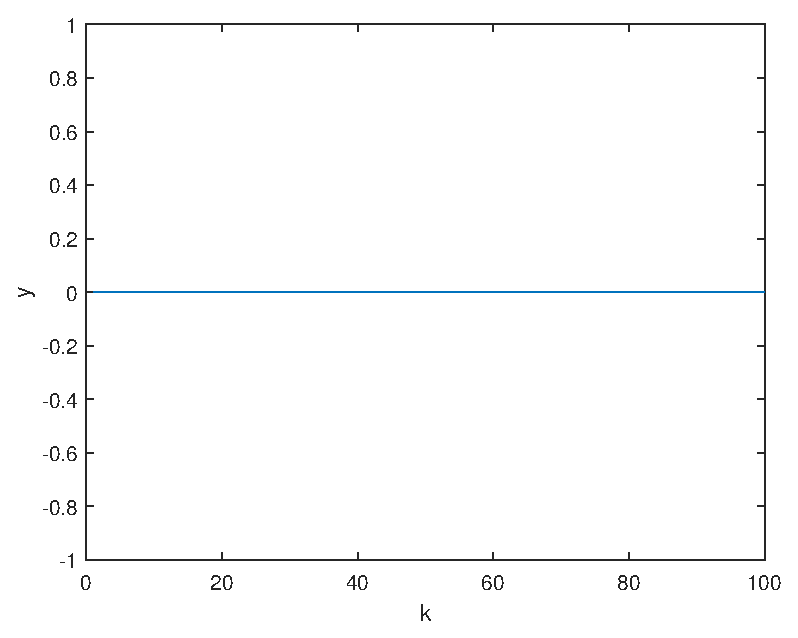
\includegraphics[scale=1]{Rys/punkt_pracy.eps}
	\caption{Odpowiedź obiektu na sterowania $u=\num{0.0}$}
\end{figure}

\part{Laboratoria}
\chapter {Pomiar w punkcie pracy}
\label{zad1l}

\section{Komunikacja z obiektem}

Komunikacja z obiektem odobywa się za pomocą funkcji napisanych w środowisku MatLab. Najprostszy program użyty w tym projekcie, który posłużył także do późniejszego pobierania odpowiedzi skokowych znajduje się poniżej (jest to fragment skryptu \verb|L3_1.m|).


%\begin{lstlisting}[style=custommatlab,frame=single]
\begin{lstlisting}[style=custommatlab]


    addpath('F:\SerialCommunication'); % add a path to the functions
    initSerialControl COM3 % initialise com port
   
    N = 420;
    step_response = zeros(N+1,1);
    i = 0;
    
    while(i<=N)
        %% obtaining measurements
        measurements = readMeasurements(1:7); % read measurements from 1 to 1
        
        %% processing of the measurements and new control values calculation
        disp([measurements(1),i]);
        step_response(i+1)=measurements(1);
        
        %% sending new values of control signals
        sendNonlinearControls(29)  % new corresponding control valuesdisp(measurements); % process measurements
      
        i=i+1;
        step_response(i)=measurements(1);
        
        waitForNewIteration(); % wait for new batch of measurements to be ready
        
    end

\end{lstlisting} 

W tym zadaniu używamy funkcji \verb|sendNonlinearControls|, który wysyła sterowanie w sposób symulujący nieliniowość obiektu. Napisany skrypt działał poprawnie, pozwala na sterowanie sygnałami G1, W1 oraz pomiar T1.

\section{Punkt pracy}

Doprowadzono obiekt do punktu pracy, tj. ustawiono wartości sygnałów W1 na 50, G1 na 29 i poczekano na ustabilizowanie obiektu (ponieważ obiekt jest rzeczywisty wahania temperatury są nieuniknione, zwłaszcza biorąc pod uwagę fakt lokalizacji stanowiska nr 4 w miejscu obok którego przechodzi dużo osób - wszelkie pomiary teraźniejsze oraz późniejsze mogą być zaburzone właśnie przez to). Wartość temperatury w punkcie pracy wynosi T1=\num{35,43}\degree C.

\chapter {Charakterystyka obiektu}
\label{zad2l}

\section {Inne punkty pracy}

W celu pobrania wartości wyjścia dla innych punktów sterowania postępowano następująco: najpierw pobudzono układ sterowaniem równym G1=\num{20} i poczekano na jego stabilizację. Następnie dokonywano skoków tej wartości sterowania o 10, aż do wartości G1=\num{80}. Przebieg eksperymentu ilustrują poniższe wykresy (skoki sterowania następowały w chwilii t=\num{0}:



\begin{figure}[h!]
	\centering
	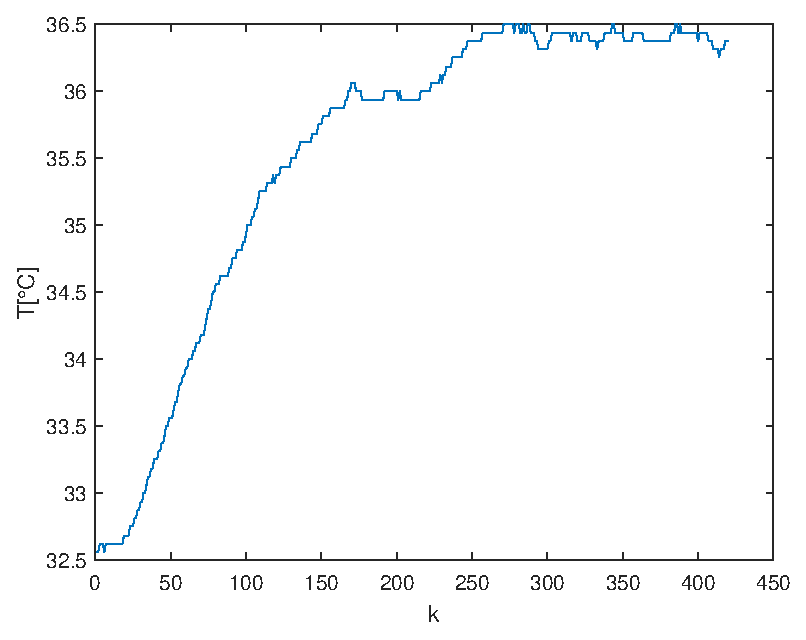
\includegraphics[scale=1]{Rys/Skok20_30.eps}
	\caption{Skok wartości sterowania z 20 do 30}
	\label{skok1}
\end{figure}

\begin{figure}[h!]
	\centering
	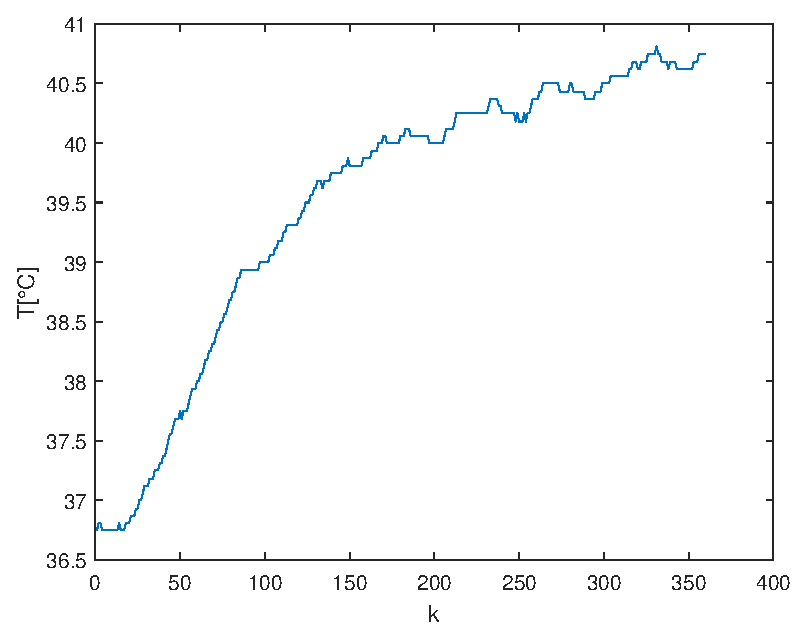
\includegraphics[scale=1]{Rys/Skok30_40.eps}
	\caption{Skok wartości sterowania z 30 do 40}
	\label{skok2}
\end{figure}

\begin{figure}[h!]
	\centering
	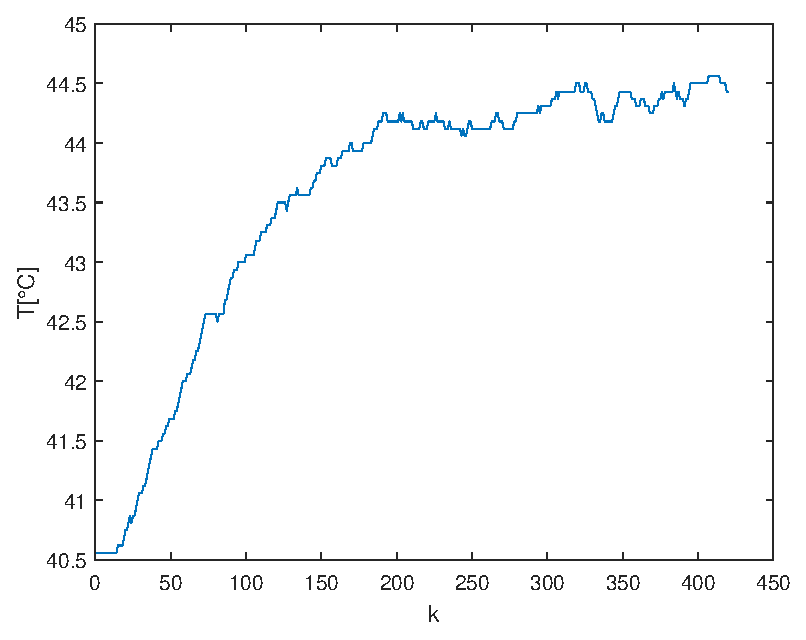
\includegraphics[scale=1]{Rys/Skok40_50.eps}
	\caption{Skok wartości sterowania z 40 do 50}
	\label{skok3}
\end{figure}

\begin{figure}[h!]
	\centering
	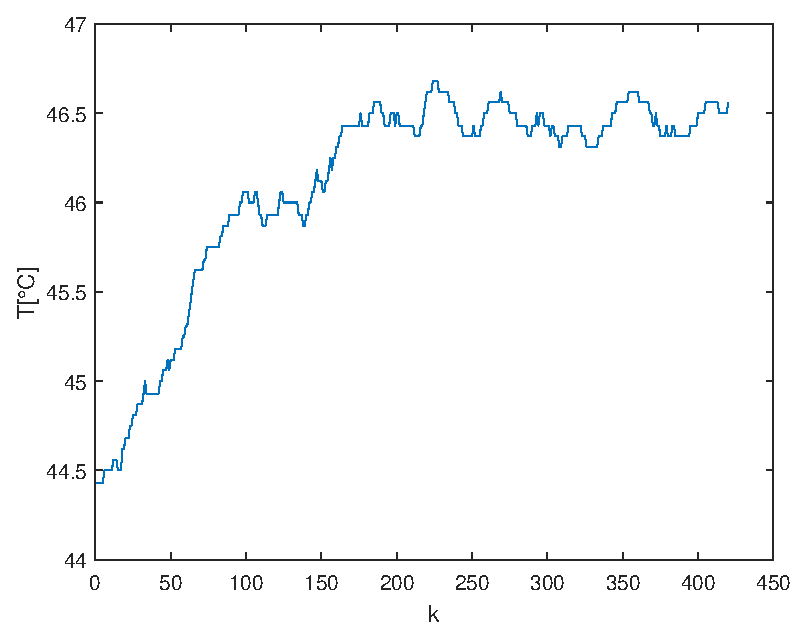
\includegraphics[scale=1]{Rys/Skok50_60.eps}
	\caption{Skok wartości sterowania z 50 do 60}
	\label{skok4}
\end{figure}

\begin{figure}[h!]
	\centering
	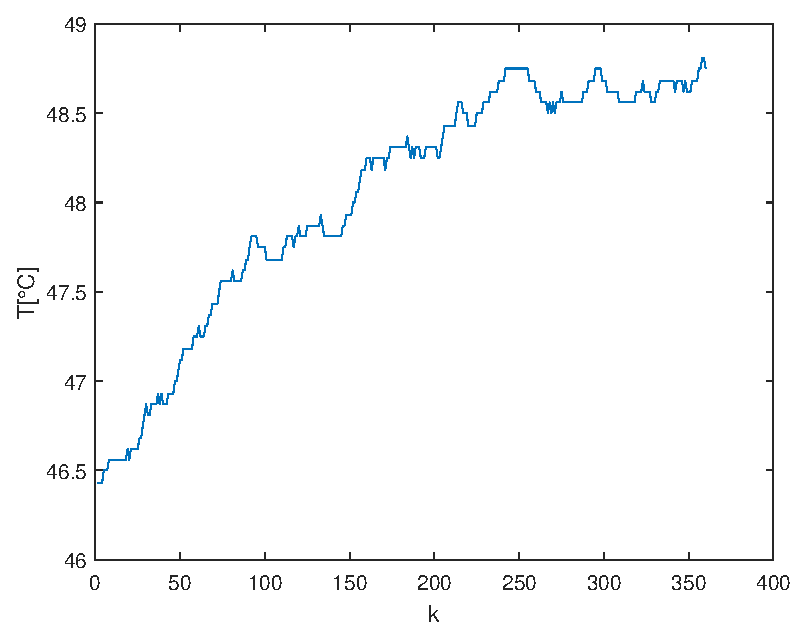
\includegraphics[scale=1]{Rys/Skok60_70.eps}
	\caption{Skok wartości sterowania z 60 do 70}
	\label{skok5}
\end{figure}

\begin{figure}[h!]
	\centering
	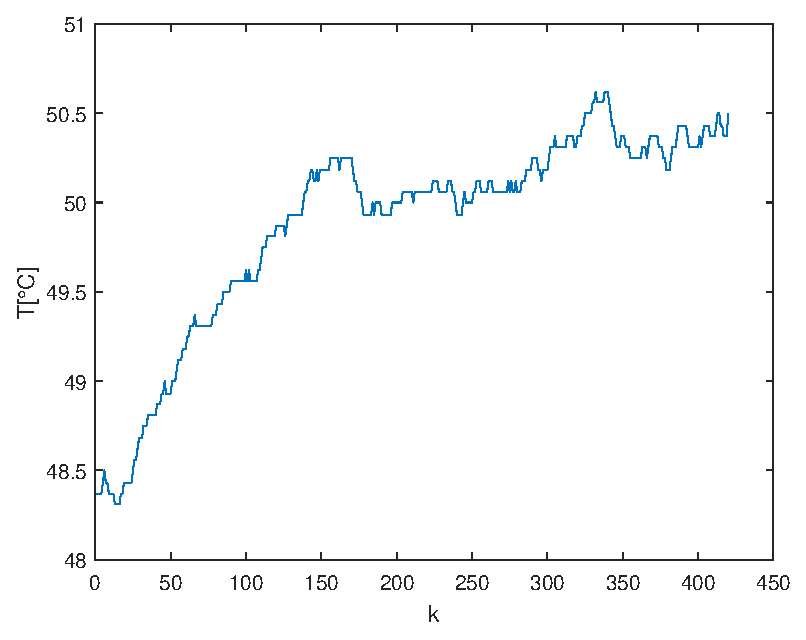
\includegraphics[scale=1]{Rys/Skok70_80.eps}
	\caption{Skok wartości sterowania z 70 do 80}
	\label{skok6}
\end{figure}

\FloatBarrier

Wyniki przedstawiono w tabeli:

\begin{center}
 \begin{tabular}{ | m{1cm}| m{1cm} | }
 \hline
 G1[\%] & T[\degree C]   \\
 \hline
 20 & \num{32,43}   \\ 
 \hline
 30 & \num{36,62 }  \\
 \hline
 40 & \num{40,75}  \\
 \hline
 50 & \num{44,31} \\
 \hline
 60 & \num{46,5}  \\ 
 \hline
 70 & \num{48,68}  \\ 
 \hline
 80 & \num{50,56}  \\
 \hline


\end{tabular}
\end{center}


\section{Charakterystyka statyczna obiektu}

Charakterystykę statyczną obiektu w przedziale sterowań G1 od 20 do 80\% przedstawiono na wykresie \ref{stat}:

\begin{figure}[h!]
	\centering
	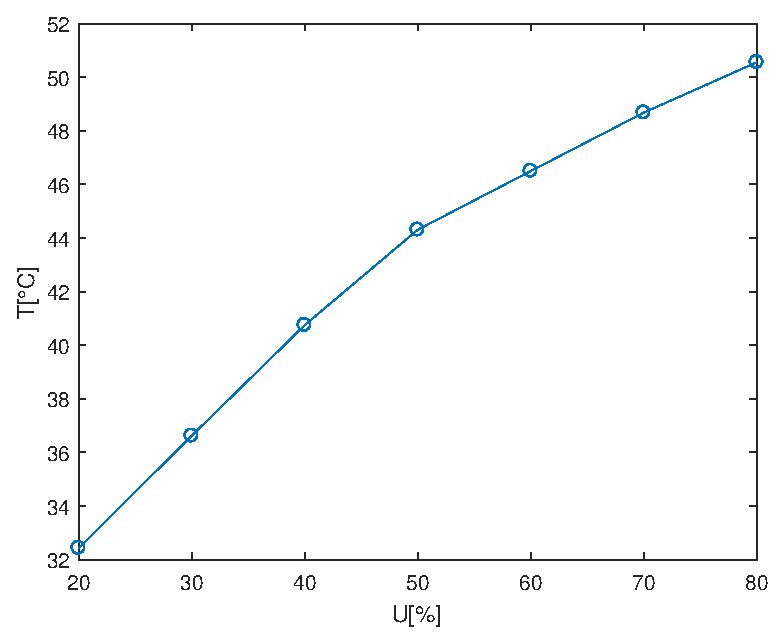
\includegraphics[scale=1]{Rys/Char_stat.eps}
	\caption{Charakterystyka statyczna obiektu}
	\label{stat}
\end{figure}


\section{Wzmocnienie statyczne}

Z wykresu charakterystyki liniowej można stwierdzić, że obiekt nie jest całkowicie liniowy, występuje załamanie charakterystyki w punkcie U=\num{50}\%. Jednak obiekt jest kawałkami liniowy, przejawia właściwości liniowe w przedziale \num{20}-\num{50}\% oraz inne  właściwości liniowe w przedziale \num{50}-\num{80}\% - na tych odcinkach obiekt zachowuje się praktycznie w sposób liniowy. Dlatego też możemy policzyć wzmocnienie statyczne obiektu w tych przedziałach sterowania:

\begin{equation}
K_{\num{20}-\num{50}\%}= \frac{Y(50)-Y(20)}{50-20}=\frac{44,31-32,43}{50-20}=0,396
\label{zad2_wzm_statyczne_wzor1}
\end{equation}


\begin{equation}
K_{\num{50}-\num{80}\%}= \frac{Y(80)-Y(50)}{80-50}=\frac{50,56-44,31}{80-50}\approx 0,208
\label{zad2_wzm_statyczne_wzor2}
\end{equation}



\chapter{Zastosowanie tradycyjnych regulatorów PID i DMC}




\section{Regulator PID}

\subsection{Postępowanie}

Zarówno w przypadku regulatora PID oraz DMC zostaną użyte skrypty  ( \verb|doFuzzyPID.m|  \verb|doFuzzyDMC.m|) z odpowiednio ustawionym parametrem odpowiadającym za typ regulatora. Jedyna zmiana względem projektu nr 1 nastąpi w wysyłaniu sterowania do obiektu, gdzie funkcję \verb|sendControls| zastępujemy funkcją \verb|sendNonlinearControls|, która ma na celu symulację braku liniowości obiektu na całym obszarze wartości sterowań. 

\subsection{Wyniki symulacji}

Wyniki symulacji przestawiono na wykresie \ref{naiwnyPID}:

\begin{figure}[h!]
	\centering
	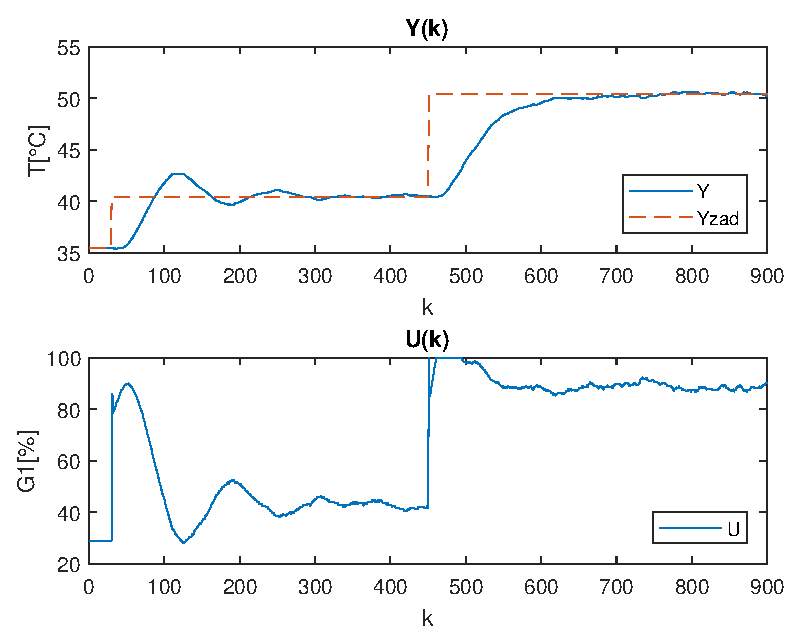
\includegraphics[scale=1]{Rys/NaiwnyPID.eps}
	\caption{Symulacja dla pojedynczego regulatora PID o parametrach $K=9,65, T_{i}=60,  T_{d}=0,17 $}
	\label{naiwnyPID}
\end{figure}


Błąd (suma kwadratów odchyłek) wyniósł E= \num{6077}.

\FloatBarrier

\section{Regulator DMC}

Wyniki symulacji przedstawiono na wykresie \ref{naiwnyDMC}:

\begin{figure}[h!]
	\centering
	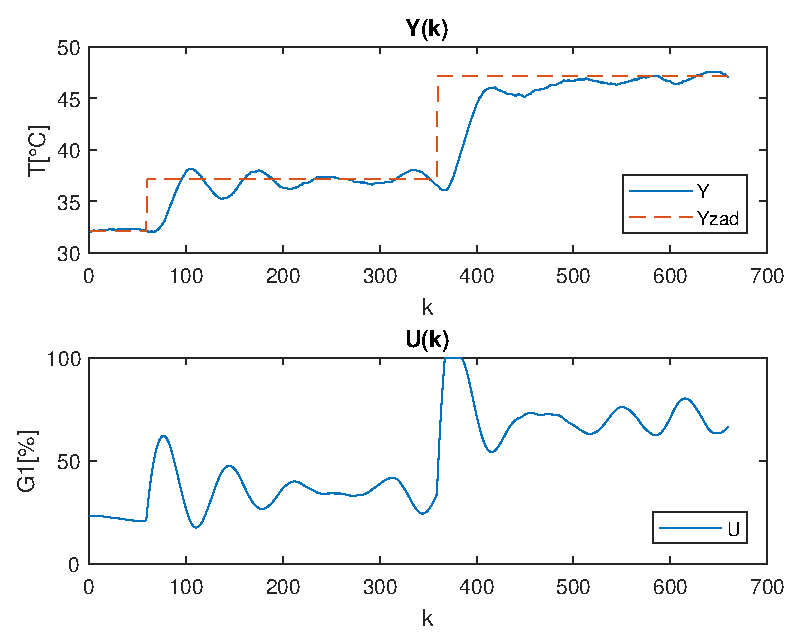
\includegraphics[scale=1]{Rys/NaiwnyDMC.eps}
	\caption{Symulacja dla pojedynczego regulatora DMC o parametrach $D=360, N=120, N_{u}=20, \lambda=1 $}
	\label{naiwnyDMC}
\end{figure}

Błąd (suma kwadratów odchyłek) wyniósł E= \num{3795} (wyniki można ze sobą porównywać mimo krótszego czasu trawnia symulacji, liczba skoków pozostała ta sama - tam są generowane głównie uchyby).

\section{Wnioski}

Pomimo że regulatory działają, temperatura zadana jest mniej więcej osiągana, jednak ich regulacja jest dosyć wolna, a wyjscie oscyluje. W celu poprawy regulacji dokonano rozmycia tych regulatorów.
\chapter{Rozmywanie regulatorów}

\section{Funkcje aktywacji}

Dla obu regulatorów dobrano identyczne funkcje aktywacjii dla trzech regulatorów lokalnych. Rozmywane one są względem wartości sterowana w poprzednim momencie. Zdecydowano się na to z dwóch powodów: po pierwsze układ może zmieniać swoje punkty pracy w zależności od warunków atmosferycznych otoczenia, rozmywanie po wyjściu naraża nas na wpływ takich odchyleń i spadek jakości regulacji; po drugie nieliniowość na obiekcie jest wprowadzana sterowaniem, tzn. obiekt (według tego co ustalono na projektach 1 oraz 2) jest w miarę liniowy, a jego właściwości nie mogły się zmienić, nieliniowość narzucana jest przez funkcję \verb|sendNonlinearControls|, która jakoby przerabia sterowanie tak, aby układ zachowywał się jak nieliniowy. \\

Pierwszy regulator lokalny będzie aktywny głównie w przedziale 0-50\% (na tym przedziale obiekt zachowuje się jak liniowy), drugi w przedziale 45-55\%, a trzeci głównie w przedziale 50-100\%, patrz rysunek \ref{fun_przyn}. Na tym etapie warto wspomnieć, iż regulator nr 2 umieszczany jest tylko w celu zaspokojenia potrzeb polecenia, sama charakterystyka wskazuje na użycie jedynie dwóch regulatorów lokalnych. Wszelkie próby dostajania regulatorów rozmytych mogą kończyć się fiaskiem z uwagi właśnie na ten sztucznie wytworzony regulator lokalny (zwłaszcza w przypadku regulatora DMC).

\begin{figure}[h!]
	\centering
	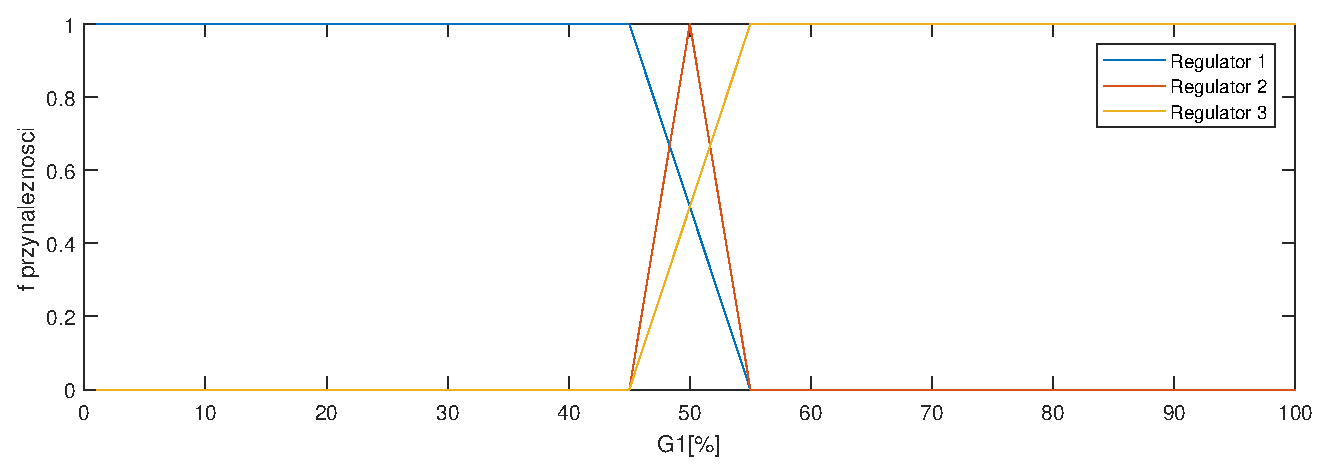
\includegraphics[scale=0.75]{Rys/Przynaleznosc.eps}
	\caption{Funkcje aktywacji regulatorów lokalnych}
	\label{fun_przyn}
\end{figure}

\FloatBarrier

\section {Rozmyty regulator PID}

\subsection{Algorytm}

Algorytm działa bardzo podobnie do tego z projektu pierwszego, tylko że każde wyjście trzech regulatorów lokalnych jest ważone przez odpowiadającą mu wartość funkcji aktywacji. Poglądowy algorytm programu porównawczego obsługującego zarówno rozmytą jak i nierozmytą wersję algorytmu wraz z bardziej szczegółowym omówieniem w postaci komentarzy został umieszczony poniżej:



\begin{lstlisting}[style=custommatlab,frame=single,label={zad4_sim_lst},caption={Implementacja regulatora PID},captionpos=b]

% Inicjalizacja polaczenia
addpath('F:\SerialCommunication'); % add a path to the functions
initSerialControl COM3 % initialise com port

% Typ regulatora
regulator=1;         

% Inicjalizacja parametrow
K=[10 10 20];
Ti=[60 60 60];
Td=[0 0 0];
T=1; 
% Inicjalizacja wskaznika jakosci
error=0;
% Inicjalizacja czasu trwania symluacji
sim_len=900;

% Parametry dyskretnego PIDa
for i=1:3
r0(i)=K(i)*(1+T/(2*Ti(i))+Td(i)/T);
r1(i)=K(i)*(T/(2*Ti(i))-2*Td(i)/T-1);
r2(i)=K(i)*Td(i)/T;
end

% Inicjalizacja
Y=zeros(sim_len,1);
U=zeros(sim_len,1);
e=zeros(sim_len,1);
y=zeros(sim_len,1);
u=zeros(sim_len,1);
Yzad=zeros(sim_len,1);
kk=linspace(1,sim_len,sim_len)';

% Zakladamy ze przed rozpoczeciem symulacji obiekt znajdowal sie w punktu pracy
Ypp=readMeasurements(1);
Upp=29;
Y(1:30)=Ypp;
U(1:30)=Upp;

% Inicjalizacja horyzontu wartosci zadanych
Yzad(1:sim_len/3-1)=Ypp+5;
Yzad(sim_len/3:2*sim_len/3-1)=Ypp+15;
Yzad(2*sim_len/3:sim_len)=Ypp;

% Ograniczenia U
Umin=0;
Umax=100;
umin=Umin-Upp;
umax=Umax-Upp;

% Glowna petla programu
for i=31:sim_len
% Odczyt wartosci temperatury
measurements = readMeasurements(1:7); 
Y(k)=measurements(1)
% Rzutowanie wzgledem wartosci punktu pracy
y(k)=Y(k)-Ypp;
% Liczenie uchybu i uaktualnienie wskaznika jakosci
e(k)=Yzad(k)-Y(k);
error=error+e(k)^2;
% Wyliczenia wartosci funkcji aktywacji
w=f_przyn(U(k-1));

% Uzycie PIDa to wyliczenia strerowania
%Jesli regulator jest nierozmyty przyjmujemy pierwsze elementy macierzy jako parametry
if regulator==1
u_wyliczone=r2(1)*e(k-2)+r1(1)*e(k-1)+r(1)*e(k)+u(k-1);

else
    for q=1:3
        u_wyliczone=u_wyliczone+w(q)*(r2(q)*e(k-2)+r1(q)*e(k-1)+r0(q)*e(k)+u(k-1));
    end
end

% Rzutowanie ograniczen na wartosc sterowania
if u_wyliczone<umin
u_wyliczone=umin;
elseif u_wyliczone>umax
u_wyliczone=umax;
end
u(k)=u_wyliczone;
% Rzutowanie sterowania wzgledem punktu pracy
U(k)=u_wyliczone+Upp;
% Wyslanie sterowania do regulatora
sendNonlinearControls(U(k))
end
\end{lstlisting} 


\subsection{Przykładowe PIDy}

W celu weryfikacji poprawności napisanego algorytmu przesymulowano obiekt dla parametrów bardzo zbliżonych do tych znalezionych w projekcie nr 1. Stanowiły one także dobry punkt wyjścia do dalszego strojenia. Jako, że przebieg był praktycznie analogiczny do tego znalezionego w zadaniu 3, nie zamieszczano go ponownie.\\

W celu poprawienia jakości regulacji, w pierwszym kroku zdecydowano się na zwiększenia wzmocnień regulatorów lokalnych 2 oraz 3, tam gdzie były największe problemy z szybkością regulacji.

\subsubsection{$K_{1}=\num{9,65},T_{i1}=\num{60},T_{d1}=\num{0,17}, K_{2}=\num{14},T_{i2}=\num{60},T_{d2}=\num{0,17}, K_{3}=\num{20},T_{i3}=\num{60},T_{d3}=\num{0,17}$ }




\begin{figure}[h!]
	\centering
	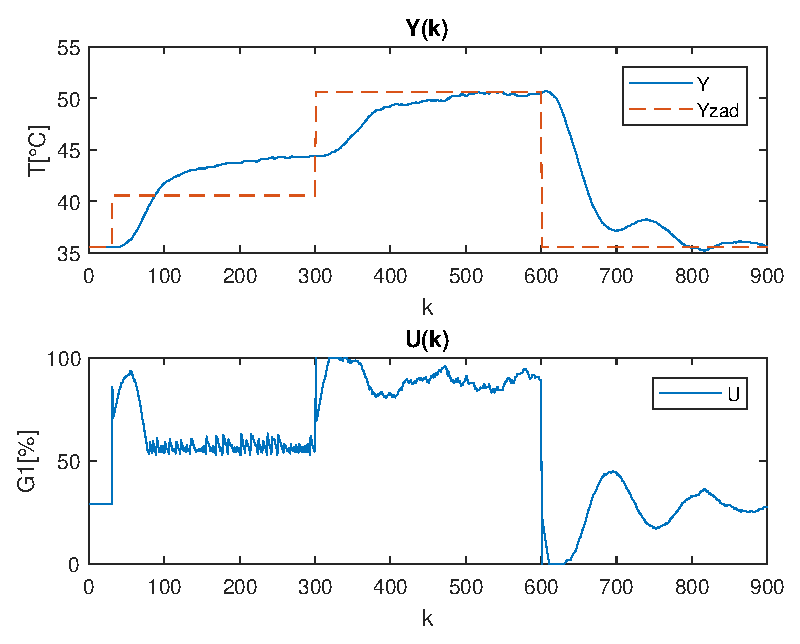
\includegraphics[scale=1]{Rys/PID2.eps}
	\caption{Symulacja regulatora rozmytego nr 1}
	\label{pid2}
\end{figure}

Widać, że regulator zachowuje się bardzo źle zwłaszcza w okolicach drugiego skoku wartości zadanej. Wynika to z faktu, iż punkt ten znajduje się blisko punktu przełączania regulatorów (sterowanie okołow wartości 50) i pozostaje w sferze aktywacji regulatora lokalnego nr 2. Wartość błędu całkowitego jest równa $E_{c}=\num{14397}$, a dla ocinka porównywalnego z wcześniejszym (niekompletnym) eksperymentem dla regulatora nierozmytego E=\num{4693,3}. O ile sama wartość błędu zmalała, wynika to bardziej z faktu iż w przypadku skoku wartości zadanej o 15 stopni regulator już znajdował się bliżej tego punktu i naliczał mniejsze kary (które są kwadratem odchyłki). Regulacja nie poprawiła się. W następnym kroku zdecydowano się na zbliżenie parametrów regulatora lokalnego nr 2 do regulatora nr 1 oraz sprawdzenie jak regulator zachowuje się po całkowitym odłączeniu członu różniczkującego.

\FloatBarrier

\subsubsection{$K_{1}=\num{10},T_{i1}=\num{60},T_{d1}=\num{0}, K_{2}=\num{10},T_{i2}=\num{60},T_{d2}=\num{0}, K_{3}=\num{20},T_{i3}=\num{60},T_{d3}=\num{0}$ }


\begin{figure}[h!]
	\centering
	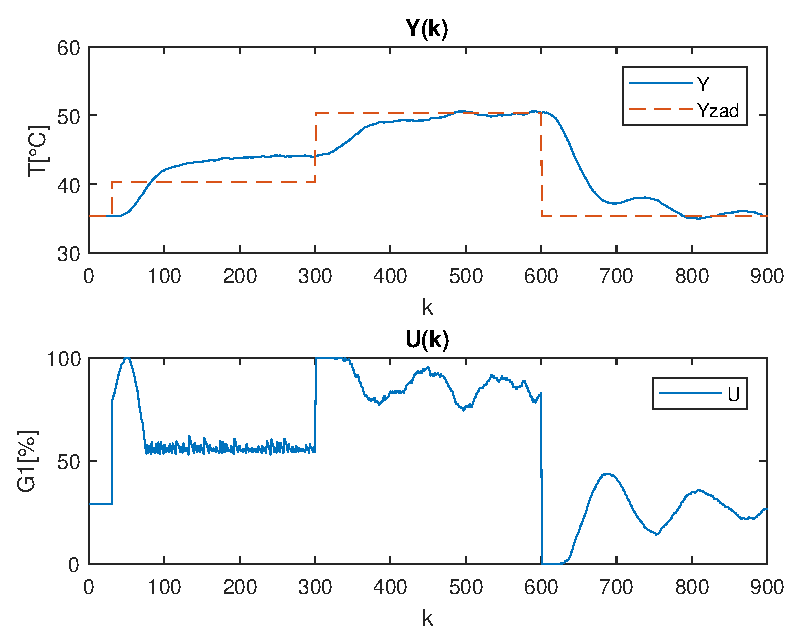
\includegraphics[scale=1]{Rys/PID3.eps}
	\caption{Symulacja regulatora rozmytego nr 2}
	\label{pid3}
\end{figure}

\FloatBarrier
Praktycznie nie nastąpiła żadna poprawa w porównaniu z poprzednim regulatorem, zachowuje się on bardzo podobnie i ma podobne problemy. Wartość błędu całkowitego jest równa $E_{c}=\num{13866}$, a dla ocinka porównywalnego z wcześniejszym (niekompletnym) eksperymentem dla regulatora nierozmytego E=\num{4638,3}, czyli są odrobinę mniejsze.



\section{DMC}

\subsection {Odpowiedzi skokowe}

Ponieważ w obszarze sterowań 20-50\% układ zachowuje się w ten sam liniowy sposób, nie powinno być różnicy, z jakiego miejsca tego przedziału weźmiemy odpowiedz skokową, analogicznie dla przedziału sterowań 50-80\%. Zdecydowano się na skoki 20->30\% oraz 50->80\%, które zdawały się mieć najlepsze własności. Do stworzenia zoptymalizowanych odpowiedzi skokowych można użyć przebiegów już wcześniej wyznaczonych. Dla regulatora lokalnego nr 2 wykonano skok sterowania 47,5->52,5\%. Przedstawiono go na rysunku \ref{skokcen}:

\begin{figure}[h!]
	\centering
	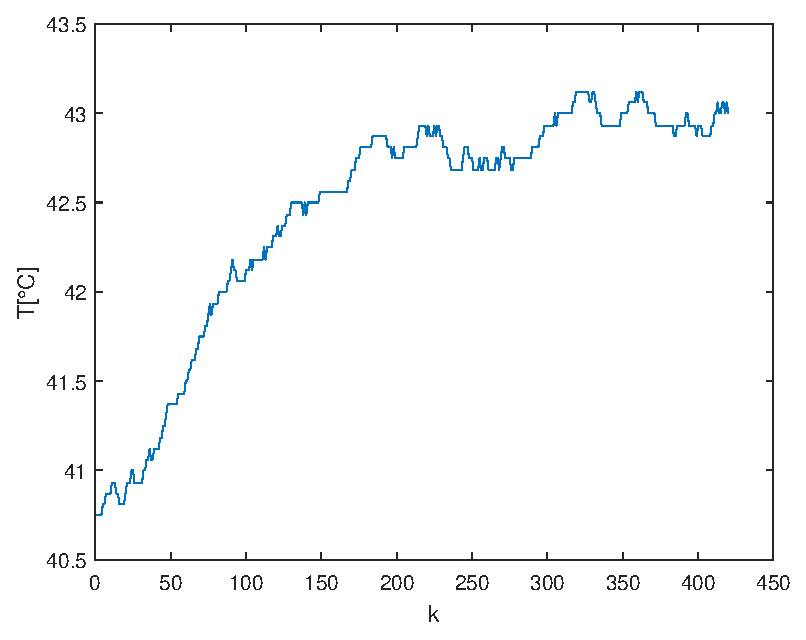
\includegraphics[scale=1]{Rys/Skokcen.eps}
	\caption{Skok wartości sterowania z \num{47,5} do \num{52,5}}
	\label{skokcen}
\end{figure}

\FloatBarrier

Następnie dokonano normalizacji wszystkich tych przebiegów w celu użycia ich w regulatorze DMC. W tym celu dokonano ich aproksymacji jako członów inercyjnych drugiego rzędu z opóźnieniem oraz dokonano ich przycięcia do wartości horyzontu dynamiki, który ustalono jako D=360. Przebiegi znormalizowanych odpowiedzi przedstawiono poniżej:


\begin{figure}[h!]
	\centering
	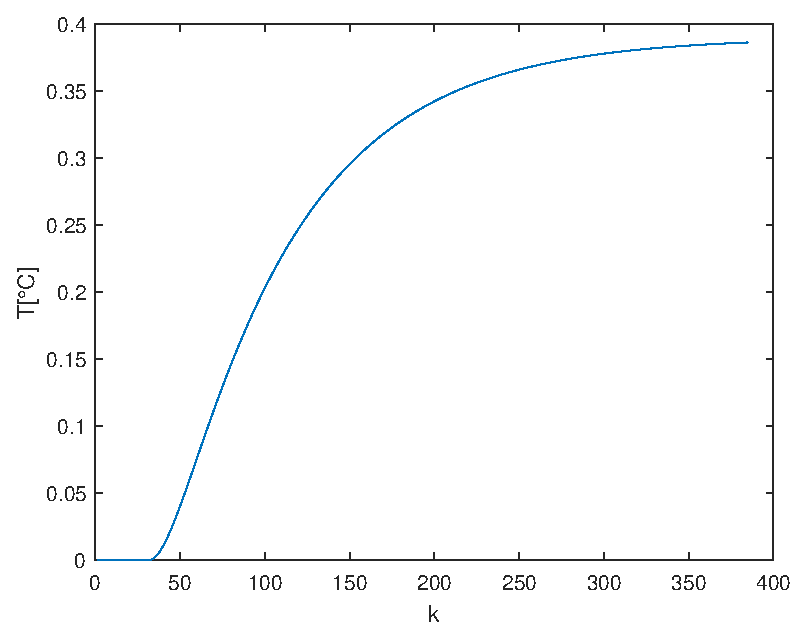
\includegraphics[scale=1]{Rys/Skok2030_approx.eps}
	\caption{Znormalizowany skok wartości sterowania z \num{20} do \num{30}}
	\label{skokn1}
\end{figure}

\begin{figure}[h!]
	\centering
	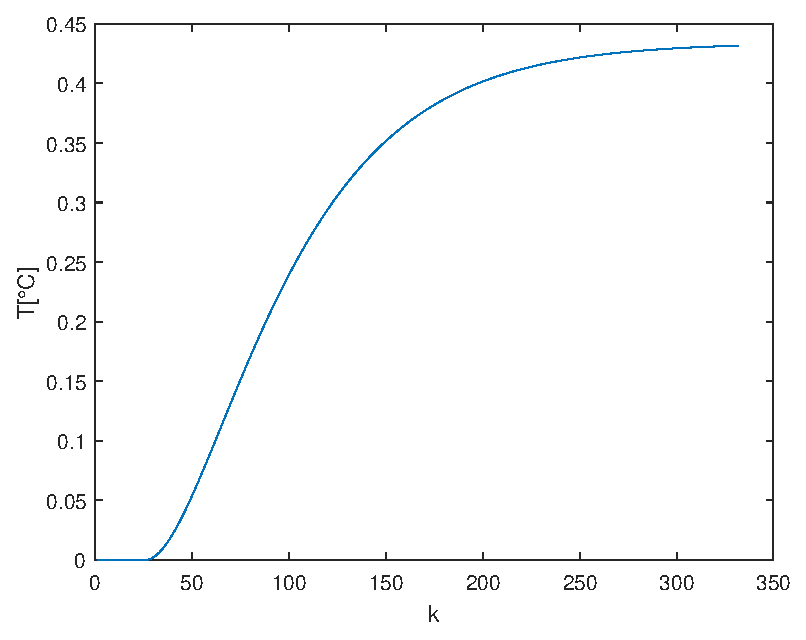
\includegraphics[scale=1]{Rys/Skokcen_approx.eps}
	\caption{Znormalizowany skok wartości sterowania z \num{47,5} do \num{52,5}}
	\label{skokn2}
\end{figure}

\begin{figure}[h!]
	\centering
	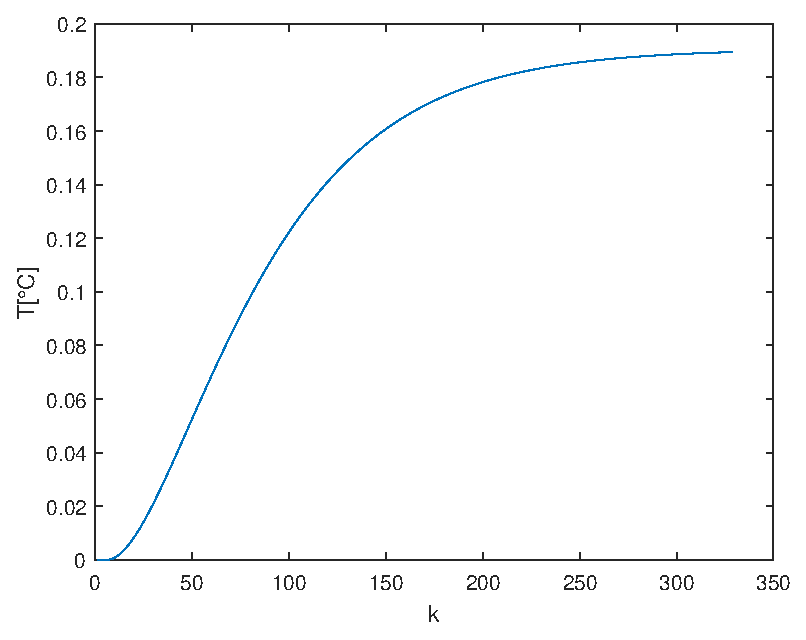
\includegraphics[scale=1]{Rys/Skok7080_approx.eps}
	\caption{Znormalizowany skok wartości sterowania z \num{70} do \num{80}}
	\label{skokn3}
\end{figure}

\FloatBarrier


\subsection {Algorytm}

\begin{lstlisting}[style=custommatlab,frame=single,label={zad4_sim_lst},caption={Implementacja regulatora DMC},captionpos=b]

% Zaladowanie odpowiedzi skokwej
load('step_response_70_80_approx');
load('step_response_20_30_approx');
load('step_response_central_approx');
% Inicjalizacja komunikacji z obiektem
addpath('F:\SerialCommunication'); 
initSerialControl COM3 

% Ustalenie maksymalnych przedzialow sterowania
Umax=100;
Umin=0;

%Ustalenie iloscie regulatorow lokalnych
il = 3;

% Ustawienie parametrow regulatora
D = 320;
N=D;
Nu=D;
lambda = [100 200 100];
    
% Inicjalizacja macierzy przechowujacych zmienne
ku = zeros(il,D-1);
ke = zeros(1,il);
deltaup=zeros(1,D-1);
deltauk = zeros(il,1);
DELTAuk = zeros(il,1);
% Zaladowanie odpowiedzi skokwych
S(:,1)=step_response_20_30_approx(1:D);
S(:,2)=step_response_central_approx(1:D);
S(:,3)=step_response_70_80_approx(1:D);

% Stworzenie macierzy M, Mp oraz wyliczenie paratmetrow ku oraz ke dla
% kazdego regulatora lokalnego
for r = 1:il
    s = S(:,r);
    
    M=zeros(N,Nu);
    for i=1:N
       for j=1:Nu
          if (i>=j)
             M(i,j)=s(i-j+1);
          end
       end
    end

    MP=zeros(N,D-1);
    for i=1:N
       for j=1:D-1
          if i+j<=D
             MP(i,j)=s(i+j)-s(j);
          else
             MP(i,j)=s(D)-s(j);
          end    
       end
    end

    I=eye(Nu);
    K=((M'*M+lambda(r)*I)^-1)*M';
    ku(r,:)=K(1,:)*MP;
    ke(r)=sum(K(1,:));
end


% Ustalenie punktu pracy
U0 = 29;
Y0 = readMeasurements(1);

% Ustalenie czasu symulacji
start = 10;
n=750;

% Inicjacja macierzy przechowujacej wyjscia, sterowanie oraz uchyby
U = U0*ones(1,n);
Y = Y0*ones(1,n);
e = zeros(1,n);

% Utworzenie horyzontu wartosci zadanej
Yz = Y;
Yz(1:10)=Y0;
Yz(11:n/3) = Y0+5;
Yz(n/3+1:2*n/3)=Y0+15;
Yz(2*n/3+1:end)=Y0;

% Petla glowna regulatora
for k = start:n
    % Odczyt wartosci wyjscia
    Y(k) = readMeasurements(1);
    % Policzenie wartosci uchybu
    e(k) = Yz(k) - Y(k);

    % Dla regulatora nierozmytego liczymy jedno sterowanie
    if regulator==1
        % Prawo regulacji
        DELTAuk(i)=ke(1)*e(k)-ku(1,:)*deltaup';   
    else
    
    % Dla regulatora rozmytego liczymy sterowanie dla kazdego regulatora
    % lokalnego
    for i = 1:il
        deltauk(i) = ke(i)*e(k)-ku(i,:)*deltaup';       
    end   
    % Polczenie wartosci funkcji aktywacji dla kazdego regulatora lokalnego
    w = f_przyn(U(k-1));
    % Przemnozenie sterowan regulatorow lokalnych przez ich wartosci
    % funkcji aktywacji
    DELTAuk = w*deltauk/sum(w);
    end
    % Przesuniecie wektora dUp
    for i = D-1:-1:2
      deltaup(i) = deltaup(i-1);
    end
    % I wpisanie do niego wyliczonego elementu
    deltaup(1) = DELTAuk;
    % Wyliczenie obecnej wartosci sterowania
    U(k) = U(k-1)+deltaup(1);
    % Uwzglednienie ograniczen na wartosc sterowania
    U(k) = max(min(U(k),Umax),Umin);
    % Korekta zmiany wartosci sterowania
    deltaup(1)=U(k)-U(k-1);
    % Wyslanie sterowania do obiektu
    sendNonlinearControls(U(k))
    
    disp([Y(k),U(k)]);
    waitForNewIteration();
end
\end{lstlisting} 

\subsection {Przykładowe DMC}

Horyzonty zgodnie z poleceniem są równe, czyli $D=N=N_{u}=360$, zmieniamy jedynie wielkości parametru $\lambda$.

\subsubsection{$\lambda_{1}=1, \lambda_{2}=1, \lambda_{3}=1$ }

\begin{figure}[h!]
	\centering
	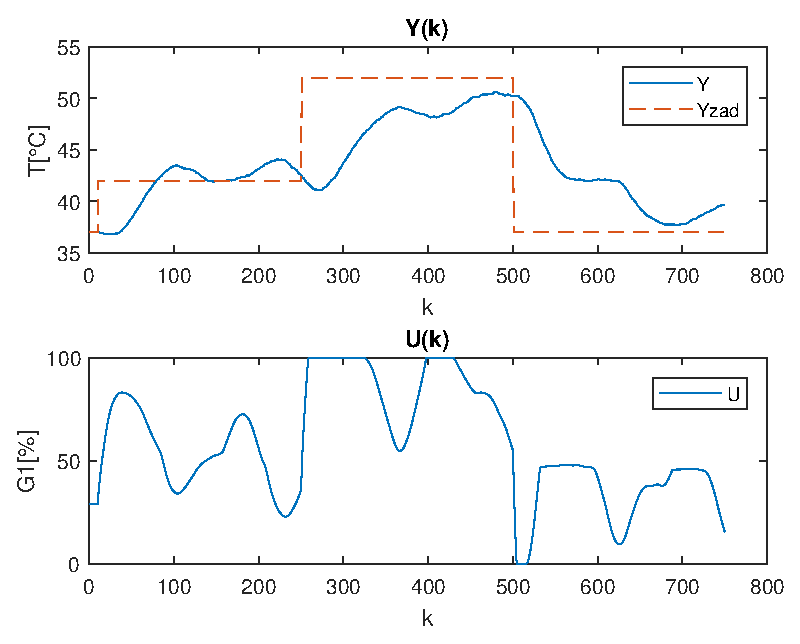
\includegraphics[scale=1]{Rys/DMC.eps}
	\caption{Rozmyty regulator nr 1}
	\label{dmc1}
\end{figure}


Wartość błędu całkowitego jest równa $E_{c}=\num{17614}$, a dla odcinka porównywalnego z wcześniejszym (niekompletnym) eksperymentem dla regulatora nierozmytego E=\num{9240}. Regulator działa źle. Sprawdzono jeszcze regulację dla zwiększonych parametrów $\lambda$. Czas laboratorium nie pozwolił na pozyskanie planowanej symulacji dla mniejszych wartości tego parametru.
\FloatBarrier

\subsubsection{$\lambda_{1}=100, \lambda_{2}=200, \lambda_{3}=100$ }


\begin{figure}[h!]
	\centering
	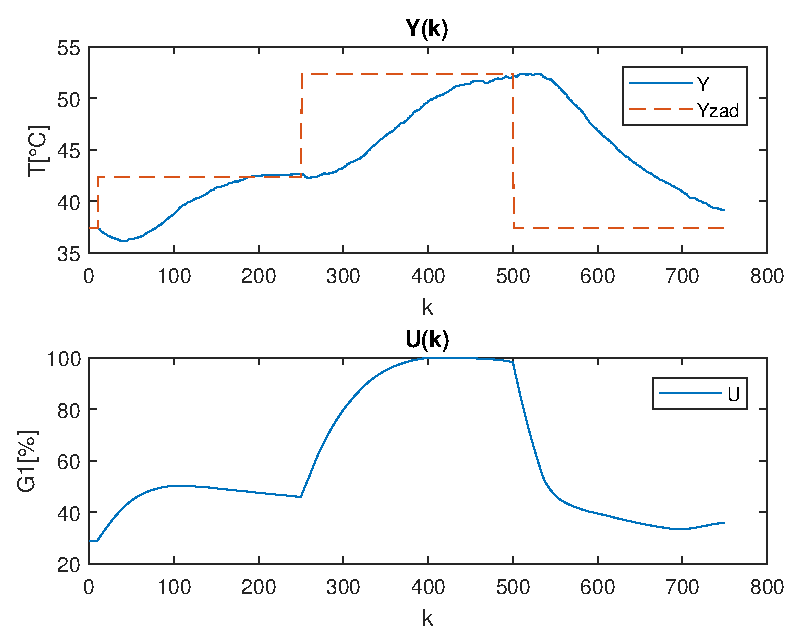
\includegraphics[scale=1]{Rys/DMC2.eps}
	\caption{Rozmyty regulator nr 2}
	\label{dmc2}
\end{figure}


Wartość błędu całkowitego jest równa $E_{c}=\num{34133}$, a dla odcinka porównywalnego z wcześniejszym (niekompletnym) eksperymentem dla regulatora nierozmytego E=\num{11814}. Regulator działa jeszcze gorzej (jest wolniejszy).
\FloatBarrier

\section{Wnioski}

Zadanie poprawy regulacji nie powiodło się - regulatry rozmyte, teoretycznie lepsze, nie przyniosły spodziewanego polepszenia jakości sterowania. Może to wynikać z: 
\begin{itemize}
  \item nieprawidłowego dobrania funkcji aktywacji poszczególnych regulatorów lokalnych, zwłaszcza drugiego, który wydaje się, że jest zbędny i tylko pogarsza regulację;
  \item w przypadku regulatora PID - niedostatkiem czasu - po przeprowadzoneniu większej ilości symulacji, możliwe, że regulator działałby dobrze;
 \item w przypadku regulatora DMC - przypadkowym użyciem nieaproksymowanych odpowiedzi skokowych (mimo posiadania ich zaproksymowanych wersji).
\end{itemize}


\appendix
\end{document}